\section{Evaluation}
We demonstrate the utility of \ApproachName~by evaluating the quality of the descriptions generated.
\ApproachName~is tailored to generate descriptions of the creation process of node-link diagrams.
To the best of our knowledge, no other application exists that can be used towards the same goal.
We believe a qualitative study is more meaningful to show the utility of \ApproachName;
thus, we conducted a qualitative user study to evaluate the quality of the descriptions.

\subsection{Study Design}
Case 2 and Case 4 were selected as evaluation datasets
because they have different types of linking conditions, visual encodings, and layouts.
An expert familiar with node-link diagram creation was invited to generate a quiz questionnaire to be used to examine, for two cases, whether participants understood node-link diagrams in two cases.
We first explained how the two node-link diagrams are created.
After that, we asked him to describe node-link diagrams in the three-step creation process.
He removed crucial information about the descriptions to generate a cloze test for each case.
The two cloze tests contain 13 vacancies and 12 vacancies respectively.

% 验证生成的句子的质量
% 李克特量表,对于四个角度以及对节点连接图的理解程度
We recruited 16 participants in the study (nine males and seven females, aged from 21 to 42, eight for Case 2 and the other eight of Case 4).
All participants are students or researchers in computer science, and eleven of them major in visualization.
We first introduce our interactive interface.
Participants were asked to read the generated descriptions interactively.
The source code and data are hidden from them.
After reading, participants were asked to finish the cloze test to check their understanding of node-link diagrams.
The expert was asked to mark cloze tests finished by participants with a full mark of five.
Participants also completed a questionnaire rating the quality of the descriptions on a five-point Likert scale regarding readability, comprehensibility, aesthetics, and usability in Table~\ref{tab:questions}.
After they finished the questionnaire, we asked them some open-ended questions for feedback and explanations.
Participants got a reward of around \$3 on completion.

% 1. 针对两个case 找一个expert帮忙写一些描述,在这个描述上挖一些空,准备一些模糊的备选项,作为quiz;
% 2. 自动生成交互式描述;
% 3. 各找12个人观看描述;回答五分量表;(readability (e.g., is it easy to read and follow the logic?),
% utility (e.g., does it help you understand this visual design?), aesthetics
% (e.g., does it look pretty and pleasant?) and attractiveness (e.g., does it
% attract your interest?).) 让被试填入。

\subsection{Results}
The participants were able to read the descriptions and fill the cloze easily.
Overall, 16 participants were satisfied with the quality of descriptions, as shown in Figure~\ref{fig:UserStudy}.
The high scores they obtained in the cloze test ($4.4, 0.57$) demonstrated that they were able to read the descriptions and obtain insights.
The questionnaires' ratings show that participants agreed that our descriptions are easy to read (readability, $4.6, 0.63$), help them understand node-link diagrams (comprehensibility, $4.5, 0.73$).
They also agreed the descriptions look pretty (aesthetics, $4.3, 0.60$) and the interaction is easy to use (usability, $4.4, 0.50$).
Several of them said that \textit{``The overall feeling is very good, it helps me quickly understand the meaning of encodings without touching the code''}.
Two participants admired the hierarchy of descriptions.
They said that \textit{``The hierarchy of descriptions helps me understand relationships of different descriptions''}.
Participants agreed our highlighting interaction enhances their comprehension: \textit{``Highlighting corresponding visual elements after I hover on descriptions makes the description easy to read. The interaction design is awesome''}.

They also gave some constructive suggestions for future improvements.
Three participants commented that more interactions could be supported in the future.
For example, they suggested that when describing coordinates, showing axes can help understand.
One participant with graph visualization experience said: \textit{``Layouts that use X and Y coordinates to encode attributes is not common, which leads to some confusion in my understanding in the beginning. But the descriptions really help me to understand such layouts.''}.
Some participants are not familiar with graph visualization; thus, they were confused about the topology-based layout.
Our description of the layout is too professional to understand.
One participant commented that our descriptions are similar to code because we highlight the key information in templates.
He asked that why colors of bars are not described in Case 4.
We explained that they only distinguish different attributes and do not encode any attribute value.



\begin{table}[]
\normalsize
\caption{Questionnaire}\label{tab:questions}
\setlength{\tabcolsep}{1.8mm}
\setlength{\extrarowheight}{3pt}
    \begin{tabular}{p{2.3cm}|p{5.7cm}}
    \hline
    readability       & Is it easy to read and follow the descriptions?     \\
    comprehensibility & Does it help to understand the visualization? \\
    aesthetics        & Do the descriptions look pretty and pleasant?       \\
    usability         & Is the interaction easy to use?                   \\ \hline
\end{tabular}
\end{table}

\begin{figure}
    \centering
    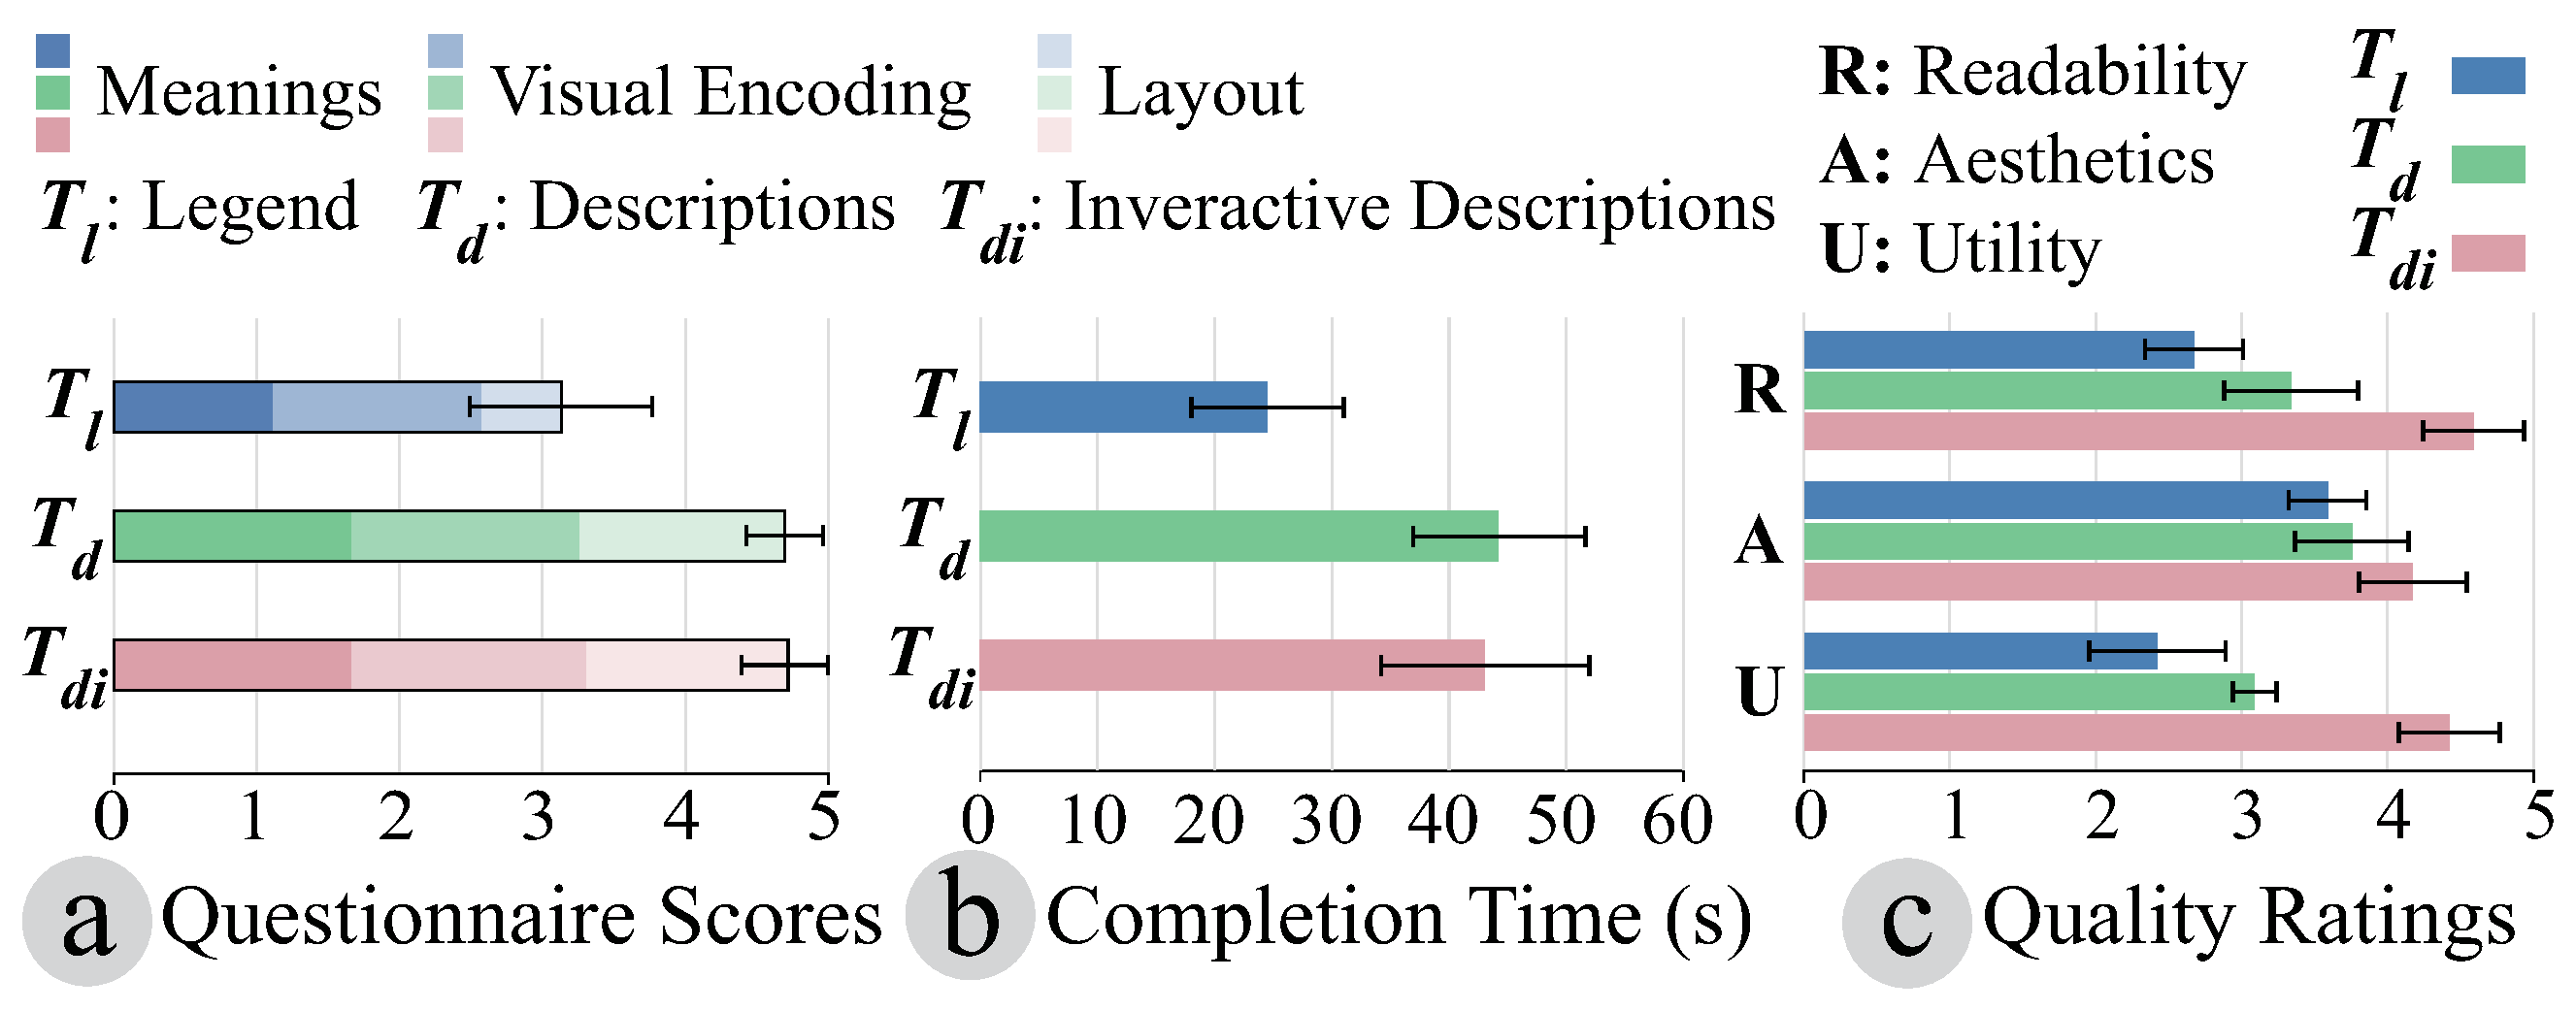
\includegraphics[width=1\columnwidth]{figures/UserStudy.eps}
    \caption{The result of our user study with $95\%$ confidence intervals.}
    \label{fig:UserStudy}
\end{figure}